\problem
\begin{question}
    Let us consider the following 1D classical heat equation
    \begin{equation}\label{heat}
    \left\{
    \begin{array}{ll}
    u_t=Du_{xx},& x\in \mathbb R, t>0, \\
    u(0,x)=\varphi(x),& x\in \mathbb R.
    \end{array}
    \right.
    \end{equation}
    where $D$ is a positive constant, $\varphi$ is a function that decays exponentially as $|x|\rightarrow \infty$.  Then the solution of (\ref{heat}) is given by
    \begin{equation}\label{heatsol}
    u(t,x)=\frac{1}{\sqrt{4\pi Dt}}\int_{\mathbb R} e^{\frac{(x-y)^2}{4Dt}}\varphi(y) dy.
    \end{equation}

    i) use the probabilistic representation for the reverse heat equation to write $u(x,t)$ in terms of a conditional expectation.  Explain this result in a physical model.  Note $D$ is not necessarily $\frac{1}{2}$;

    ii) evaluate the expectation in i) and show that it gives rise to (\ref{heatsol});

    iii) numerical studies through Monte Carlo simulations: set $D=1$ and $\varphi$ be the characteristic function such that $\varphi\equiv 1$ for $|x|<1$ and $\varphi\equiv0$ for $|x|\geq1$.  Plot the solution $u(t,x)$ by evaluating the expectation in i) for $t=0.01,0.1, 0.5$ and $1$.  This should give us four curves of $x$ which describe the evolution of $u(t,x)$.  Beautify your plots when necessary.
\end{question}
\begin{subproblem}
    \item
    For an arbitrary $T>0$, denote $v(t,x)=u(T-t,\sqrt{2D}x)$,
    then we see that
    \[v_t(t,x)=-u_t(T-t,\sqrt{2D}x),v_{xx}=2Du_{xx}(T-t,\sqrt{2D}x)\]
    thus by the heat equation of $u(t,x)$,
    \[\left\{\begin{aligned}
        &v_t+\frac{v_{xx}}{2}=0,&x\in\mathbb R,t\in[0,T)\\
        &v(T,x)=\varphi(\sqrt{2D}x),&x\in\mathbb R
    \end{aligned}\right.\]

    Then we have from It\^o's lemma that
    \[\diff v(t,W_t)=\left(v_t+\frac{v_{xx}}{2}\right)\diff t
    +v_x\diff W_t=v_x\diff W_t\]
    which gives us
    \[v(T,W_T)-v(t,W_t)=\int_t^Tv_x\diff W_t\]
    Taking conditional expectation with $W_t=x$ on BHS gives us
    \[E[v(T,W_T)|W_t=x]-v(t,x)=0\]
    i.e.,
    \[v(t,x)=E[v(T,W_T)|W_t=x]=E[\varphi(\sqrt{2D}W_T)|W_t=x]\]
    Therefore\footnote{The expression of $u(t,x)$ only contains $T$
    formally, on which it does not depend indeed. For any $t$,
    one just needs to choose a $T$ greater than it.},
    \[u(t,x)=v(T-t,x/\sqrt{2D})
    =E[\varphi(\sqrt{2D}W_T)|W_{T-t}=x/\sqrt{2D}]\]
    which is the probabilistic representation. 

    \item
    \begin{proof}
        We have from the independent increments of Brownian motion
        that
        \[\begin{aligned}
            &E[\varphi(\sqrt{2D}W_T)|W_{T-t}=x/\sqrt{2D}]\\
            =&E[\varphi(x+\sqrt{2D}(W_T-W_{T_t})|W_{T-t}=x/\sqrt{2D}]\\
            =&E[\varphi(x+\sqrt{2D}(W_T-W_{T_t}))]
        \end{aligned}\]
        Then
        \[\begin{aligned}
            u(t,x)&=E[\varphi(x+\sqrt{2D}(W_T-W_{T-t}))]\\
            &=\int_{\mathbb R}\varphi(x+\sqrt{2D}z)\frac{\e^{-\frac{z^2}{2t}}}{\sqrt{2\pi t}}\diff z\\
            (y=x+\sqrt{2D}z)\quad&=\frac{1}{\sqrt{2\pi t}}
            \int_{\mathbb R}\varphi(y)\e^{-\frac{1}{2t}\left(\frac{y-x}{\sqrt{2D}}\right)^2}
            \frac{\diff y}{\sqrt{2D}}\\
            &=\frac{1}{\sqrt{4\pi Dt}}
            \int_{\mathbb R}\e^{-\frac{(x-y)^2}{4Dt}}\varphi(y)\diff y
        \end{aligned}\]
        as $W_T-W_{T-t}\sim\mathcal N(0,t)$.
    \end{proof}

    \item
    See \cref{fig:prob sol}.
    \begin{figure}[h]
        \centering
        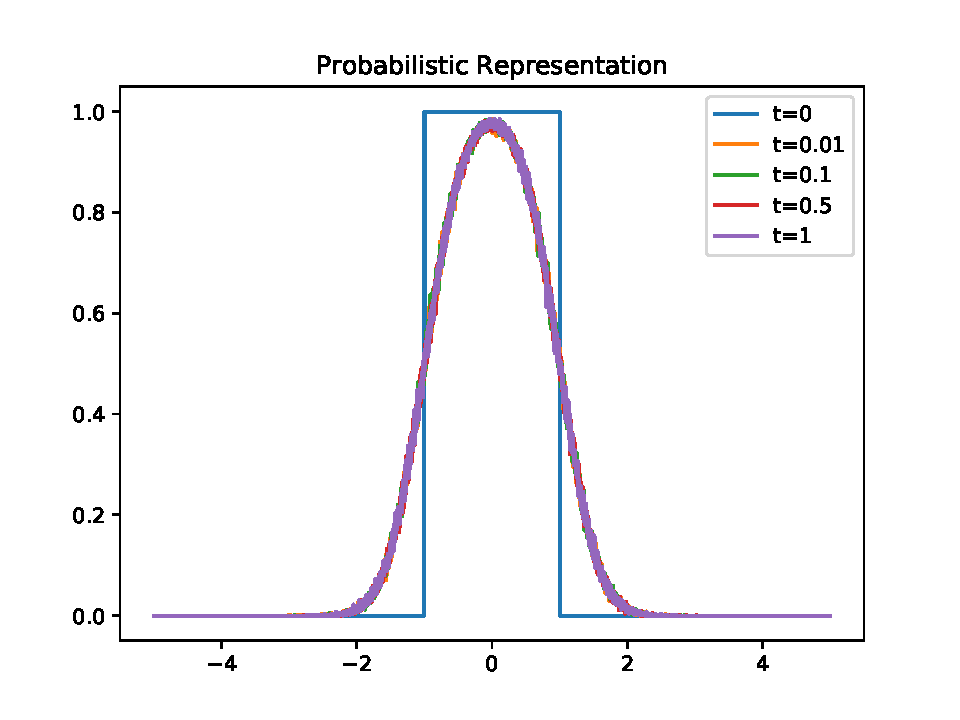
\includegraphics[width=\textwidth]{prob-sol}
        \caption{Numerical Solution by Monte Carlo Simulation}
        \label{fig:prob sol}
    \end{figure}
\end{subproblem}

\problem
\begin{question}
    Find the It\^o diffusion corresponding to the generator $Af(x)=f''(x)+f'(x)$;
\end{question}
Denote that $X_t$ is an It\^o process
 driven by $\diff X_t=\mu(t,W_t,X_t)\diff t+\sigma(t,W_t,X_t)\diff W_t$
with initial value $X_0=x$.
Then we have from It\^o's lemma
that
\[\diff f(X_t)=f'(X_t)\diff X_t+f''(X_t)\frac{1}{2}(\diff X_t)^2
=\left(\mu f'+\frac{1}{2}\sigma^2 f''\right)\diff t+\sigma f'\diff W_t\]
which gives us
\[f(X_t)=f(X_0)+\int_0^t\left(\mu f'+\frac{1}{2}\sigma^2 f''\right)\diff s
+\int_0^t\sigma f'\diff W_s\]
Taking expectation on BHS yields
\[E[f(X_t)]=f(x)+\int_0^tE\left[\mu f'+\frac{1}{2}\sigma^2 f''\right]\diff s\]
Therefore,
\[\begin{aligned}
    Af(x)&=\lim_{t\to 0^+}\frac{E[f(X_t)]-f(x)}{t}\\
    &=\left.E\left[\mu f'+\frac{1}{2}\sigma^2 f''\right]\right|_{t=0}\\
    &=\mu(0,0,x) f'(x)+\frac{1}{2}\sigma^2(0,0,x) f''(x)
\end{aligned}\]
Hence we can choose any function $\mu(t,w,x),\sigma(t,w,x)$
s.t. $\mu(0,0,x)=1,\sigma^2(0,0,x)=2$ to
our goal.

\problem
\begin{question}
    Let $X_t$ and $Y_t$ be two one--dimensional independent It\^o diffusions with infinitesimal generators $A_X$ and $A_Y$.  Prove that the infinitesimal generator of $Z_t=(X_t,Y_t)$ is $A_Z=A_X+A_Y$.
\end{question}
\begin{proof}
    Denote that the two independent It\^o diffusion are driven by
    \[\diff X_t=\mu_1\diff t+\sigma_1\diff W_t^{(1)},
    \diff Y_t=\mu_2\diff t+\sigma_2\diff W_t^{(2)}\]
    which start from from $x,y$ respectly,
    where $W_t^{(1)},W_t^{(2)}$ are two independent Brownian motion.
    And we have from It\^o's lemma that
    \[\diff f(X_t,Y_t)=f_x\diff X_t+f_y\diff Y_t+\frac{1}{2}f_{xx}(\diff X_t)^2
    +\frac{1}{2}f_{yy}(\diff Y_t)^2\]
    as independence implies $\diff X_t\diff Y_t=0$. By forward calculation, we obtain
    $\diff f(X_t,Y_t)$ as
    \[\diff f(X_t,Y_t)=\begin{aligned}[t]
    &\left(\mu_1f_x+\frac{\sigma^2_1}{2}f_{xx}
    +\mu_2f_y+\frac{\sigma^2_2}{2}f_{yy}\right)\diff t\\
    &+\sigma_1f_x\diff W_t^{(1)}+\sigma_2f_y\diff W_t^{(2)}
    \end{aligned}\]
    which gives us
    \[E[f(X_t,Y_t)]-f(x,y)=E\left[\int_0^t
    \left(\mu_1f_x+\frac{\sigma_1^2}{2}f_{xx}
    +\mu_2f_y+\frac{\sigma_2^2}{2}f_{yy}\right)\diff t
    \right]\]
    impling that
    \[\begin{aligned}
        &A_Zf(x,y)\\
        =&E\left[\left.\mu_1f_x(X_t,Y_t)+\frac{\sigma_1^2}{2}f_{xx}(X_t,Y_t)
        +\mu_2f_y(X_t,Y_t)+\frac{\sigma_2^2}{2}f_{yy}(X_t,Y_t)\right]\right|_{t=0}\\
        =&\mu_1f_x(x,y)+\frac{\sigma_1^2}{2}f_{xx}(x,y)
        +\mu_2f_y(x,y)+\frac{\sigma_2^2}{2}f_{yy}(x,y)\\
    \end{aligned}\]
    In other words,
    \[A_Z=\mu_1\frac{\partial}{\partial x}
    +\frac{\sigma_1^2}{2}\frac{\partial^2}{\partial x^2}
    +\mu_2\frac{\partial}{\partial y}
    +\frac{\sigma_2^2}{2}\frac{\partial^2}{\partial y^2}
    =A_X+A_Y\]
    as we leart from class that (by similar induction)
    \[A_X=\mu_1\frac{\partial}{\partial x}
    +\frac{\sigma_1^2}{2}\frac{\partial^2}{\partial x^2},
    A_Y=\mu_2\frac{\partial}{\partial y}
    +\frac{\sigma_2^2}{2}\frac{\partial^2}{\partial y^2}\]


\end{proof}

\problem
\begin{question}
    Consider the following parabolic equation
    \begin{equation}
    \left\{
    \begin{array}{ll}
    u_t+u_x+\frac{1}{2}u_{xx}=-1,&x\in\mathbb R,t\in(0,T),\\
    u(T,x)=0,&x\in\mathbb R.
    \end{array}
    \right.
    \end{equation}
    Represent the solution in terms of conditional expectation by
    \begin{enumerate}[label=(\alph*)]
    \item Feynman--Kac formula;
    \item infinitesimal generator;
    \end{enumerate}
    Then find the solution by evaluating this conditional expectation.  Hint: you should verify that your solution satisfies the PDE by substituting it into the equation.
\end{question}
\begin{subproblem}[(\alph*)]
    \item
    It easy to find that the functions in Feymann-Kac formula
    satisfy $\mu=\sigma=f=1,\psi=v=0$, then we have that 
    \[u(t,x)=E\left[\left.\int_t^T\diff r\right|X_t=x\right]
    =T-t\]
    where $X_t$ is an It\^o process driven by
    \[\diff X_t=\mu\diff t+\sigma\diff W_t\]

    \item
    Denote that $\mathcal A$ is an infinitesimal of
    the It\^o process driven by
    \[\diff X_t=\diff t+\diff W_t\]
    then it easy to find that
    \[\mathcal Af(t,x)=f_t+f_x+\frac{1}{2}f_{xx}\]
    To see this, just notice that by It\^o's lemma,
    \[\begin{aligned}
        \diff f(t,X_t)&=f_t\diff t+f_x\diff X_t+\frac{1}{2}f_{xx}(\diff X_t)^2\\
        &=\left(f_t+f_x+\frac{1}{2}f_{xx}\right)\diff t+f_x\diff W_t
    \end{aligned}\]
    which gives us (here we choose $s\geq t$)
    \[f(s,X_s)-f(t,X_t)=\int_t^s\left(f_t+f_x+\frac{1}{2}f_{xx}\right)\diff r
    +\int_t^s f_x\diff W_r\]
    Taking conditional expectation on BHS with $X_t=x$ yields
    \[\begin{aligned}
        E[f(s,X_s)|X_t=x]-f(t,x)&=\int_t^s E\left[\left.f_t+f_x+\frac{1}{2}f_{xx}\right|X_t=x\right]\diff r\\
        &=\int_t^s \left(f_t(t,x)+f_x(t,x)+\frac{1}{2}f_{xx}(t,x)\right)\diff r
    \end{aligned}\]
    Then we obtain our claim by the definition of infinitesimal generator
    \[\mathcal Af(t,x):=\lim_{s\to t^+}\frac{E[f(s,X_s)|X_t=x]-f(t,x)}{s-t}\]
    Hence for the solution $u(x,t)$ of the PDE, we have
    that $\mathcal Au=-1$.
    Therefore,
    \[\begin{aligned}
        E\left[u(T,X_T)|X_t=x\right]
        -u(t,x)&=
        E\left[\left.\int_t^{T}
        \mathcal Af(s,X_{s})\diff s\right|X_t=x\right]\\
        &=t-T
    \end{aligned}\]
    which gives us
    \[u(t,x)=E[u(T,X_T)|X_t=x]+T-t=T-t\]
    And it is apparent that $u(t,x)=T-t$ is the solution to the
    PDE indeed.
\end{subproblem}

\problem
\begin{question}
    Find the It\^o diffusion $X_t$ associated with the infinitesimal generator $\frac{\partial }{\partial t}+\mu x \frac{\partial }{\partial x}+\frac{1}{2}\sigma^2x^2 \frac{\partial^2}{\partial x^2}$ and then use it to find the solution to
    \begin{equation}
    \left\{
    \begin{array}{ll}
    \frac{\partial u}{\partial t}+\mu x \frac{\partial u}{\partial x}+\frac{1}{2}\sigma^2x^2 \frac{\partial^2 u}{\partial x^2}=-x,&x\in\mathbb R,t\in(0,T),\\
    u(T,x)=0,&x\in\mathbb R.
    \end{array}
    \right.
    \end{equation}
\end{question}
Denote an It\^o diffusion $X_t$ driven by
\begin{equation}
    \label{eq:a b Ito}
    \diff X_t=\alpha(t,X_t)\diff t+\beta(t,X_t)\diff W_t
\end{equation}
then the corresponded infinitesimal generator $\mathcal A$
is given by
\[\mathcal A=\frac{\partial}{\partial t}+\alpha(t,x)\frac{\partial}{\partial x}
+\frac{\beta^2(t,x)}{2}\frac{\partial^2}{\partial x^2}\]
Hence it is easy to see that we can choose
\begin{equation}
    \label{eq:param}
    \alpha(t,x)=\mu x,\beta(t,x)=\sigma x
\end{equation}
to turn $\mathcal A$ the desired.

Therefore,
\[\begin{aligned}
    E[u(T,X_T)|X_t=x]-u(t,x)
    &=E\left[\left.\int_t^T\mathcal Au(s,X_s)\diff s\right|
    X_t=x\right]\\
    &=-\int_t^TE(X_s|X_t=x)\diff s
\end{aligned}\]
which gives us
\[u(t,x)=\int_t^TE(X_s|X_t=x)\diff s\]
as $u(T,X_T)=0$.
And \cref{eq:a b Ito} together with \cref{eq:param} gives us
\[E(X_s)-E(X_t)=\mu\int_t^sE(X_r)\diff r\]
thus by solving the ODE we have $E(X_s|X_t=x)=x\e^{\mu(s-t)}$.
Finally, we obatin $u(t,x)$ as
\[u(t,x)=\int_t^Tx\e^{\mu(s-t)}\diff s
=\frac{x}{\mu}\left(\e^{\mu(T-t)}-1\right)\]

\problem
\begin{question}
    Let $\Omega \subset\mathbb R^n$, $n\geq1$, be a bounded domain with smooth boundary $\partial\Omega$.  According to PDE theory, there exists a smooth solution $u=u(x)$ of the following equation
    \begin{equation}
    \left\{
    \begin{array}{ll}
    -\frac{1}{2}\Delta u=1,&x\in\Omega,\\
    u=0,&x\in\partial \Omega.
    \end{array}
    \right.
    \end{equation}
    Prove that for each point $x\in\Omega$, $u(x)=E(\tau_x)$, where $\tau_x$ is the first time that a Brownian motion starting at $x$ hits $\partial \Omega$.
\end{question}
We know that for the Brownian motion the infinitesimal generator
$\mathcal A$ is $\Delta/2$, hence if we denote that $X_t=x+W_t$, then
we have that
\[E\left[\int_0^{\tau_x}\mathcal Au(x)\diff t\right]
=E(u(X_{\tau_x}))-E(u(X_0))\]
And we have from the PDE that $Au(x)=-1$,
and since $X_{\tau_x}\in\partial\Omega$ thus $u(X_{\tau_x})=0$,
then we obtain
\[-E\left[\int_0^{\tau_x}\diff t\right]=-u(x)\]
i.e.,
\[u(x)=E(\tau_x)\]

\problem
\begin{question}
    Consider the following equation
    \begin{equation}
    \left\{
    \begin{array}{ll}
    -\frac{1}{2}\Delta u+cu=f,&x\in\Omega,\\
    u=0,&x\in\partial \Omega,
    \end{array}
    \right.
    \end{equation}
    where $c=c(x)$ and $f=f(x)$ are smooth functions, and $c\geq0$ in $\Omega$.  Prove that, for each $x\in \Omega$,
    \[u(x)=E\Big(\int_0^{\tau_x}f(X_t)e^{-\int_0^t ic(X_s) ds}dt\Big),\]
    where $X_t=W_t+x$, i.e., the n-D Brownian motion statuting at $x$ and $\tau_x$ is the first time that $X_t$ hits $\partial \Omega$.  Hint: find $d\big(u(X_t)e^{-\int_0^t c(X_s) ds} \big)$ first and then mimic the proof of Feynman--Kac Theorem.  This is an extension of the previous problem.
\end{question}
\begin{proof}
    Denote $Y_t=u(X_t)\e^{\int_0^tc(X_s)\diff s}$,
    then $Y_0=u(x)$ and
    \[\diff Y_t=
    \begin{aligned}[t]
    u(X_t)\e^{-\int_0^tc(X_s)\diff s}(-c(X_t)\diff t)
    +\e^{\int_0^tc(X_s)\diff s}(\diff u(X_t))\\
    +\diff(u(X_t))\e^{-\int_0^tc(X_s)\diff s}(-c(X_t))\diff t
    \end{aligned}\]
    And we know that
    \[\diff(u(X_t))=u'(X_t)\diff X_t+\frac{1}{2}u''(X_t)(\diff X_t)^2
    =u'(X_t)\diff W_t+\frac{1}{2}u''(X_t)\diff t\]
    Therefore,
    \[\begin{aligned}
        \diff Y_t&=
        \left(\frac{1}{2}u''(X_t)-u(X_t)c(X_t)\right)\e^{-\int_0^tc(X_s)\diff s}\diff t
        +u'(X_t)\e^{-\int_0^tc(X_s)\diff s}\diff W_t\\
        &=\left(-f(X_t)\diff t+u'(X_t)\diff W_t\right)\e^{-\int_0^tc(X_s)\diff s}
    \end{aligned}\]
    where the last identity is due to the PDE.
    Integral over $[0,\tau_x]$ and taking expectation gives us
    \[E(Y_{\tau_x})-E(Y_0)
    =-E\left[\int_0^{\tau_x}f(X_t)\e^{-\int_0^{\tau_x}c(X_s)\diff s}\diff t\right]\]
    Note that $Y_0=u(x)$ and we have from boundary condition that $Y_{\tau_x}=0$,
    finally we obtain $u(x)$ as
    \[u(x)=E\left[\int_0^{\tau_x}f(X_t)\e^{-\int_0^{\tau_x}c(X_s)\diff s}\diff t\right]\]
\end{proof}

\appendix
\section{Python Code}
\lstinputlisting[language=Python]{montecarlo.py}